\documentclass[aspectratio=169,10pt]{beamer}

\usetheme{Madrid}
\setbeamertemplate{navigation symbols}{}
\setbeamertemplate{footline}[frame number]
\usepackage{hyperref}
\usepackage{amsmath}
\usepackage{amssymb}
\usepackage{array}
\usepackage{booktabs}
\usepackage{graphicx}
\usepackage{tabularx}
\usepackage{tikz}
\usetikzlibrary{arrows.meta,calc,positioning}

\graphicspath{{../../figures/}{../../figures_registration/}{../../data/}}

\definecolor{LectureBlue}{RGB}{13,76,100}
\definecolor{LectureTeal}{RGB}{0,118,122}
\definecolor{LectureGold}{RGB}{194,142,37}
\definecolor{Slate}{RGB}{58,68,84}
\definecolor{SoftGray}{RGB}{245,247,249}

\setbeamercolor{title}{fg=LectureBlue}
\setbeamercolor{subtitle}{fg=Slate}
\setbeamercolor{frametitle}{fg=LectureBlue,bg=LectureBlue!8}
\setbeamercolor{structure}{fg=LectureBlue}
\setbeamercolor{block title}{fg=white,bg=LectureBlue}
\setbeamercolor{block body}{fg=black,bg=SoftGray}
\setbeamercolor{alerted text}{fg=LectureGold}

\renewcommand{\arraystretch}{1.12}

\title{Image Registration: Principles, Methods, and Applications}
\subtitle{Lecture for Data Science Students}
\author{}
\date{June 2026}

\begin{document}

% Title Frame
\begin{frame}[plain]
\begin{columns}[c,onlytextwidth]
\column{0.55\textwidth}
{\usebeamerfont{title}\color{LectureBlue}\inserttitle\par}
\vspace{0.4em}
{\usebeamerfont{subtitle}\color{Slate}\insertsubtitle\par}
\vspace{1.5em}
{\small Data Science Lecture Series}
\column{0.41\textwidth}
\centering
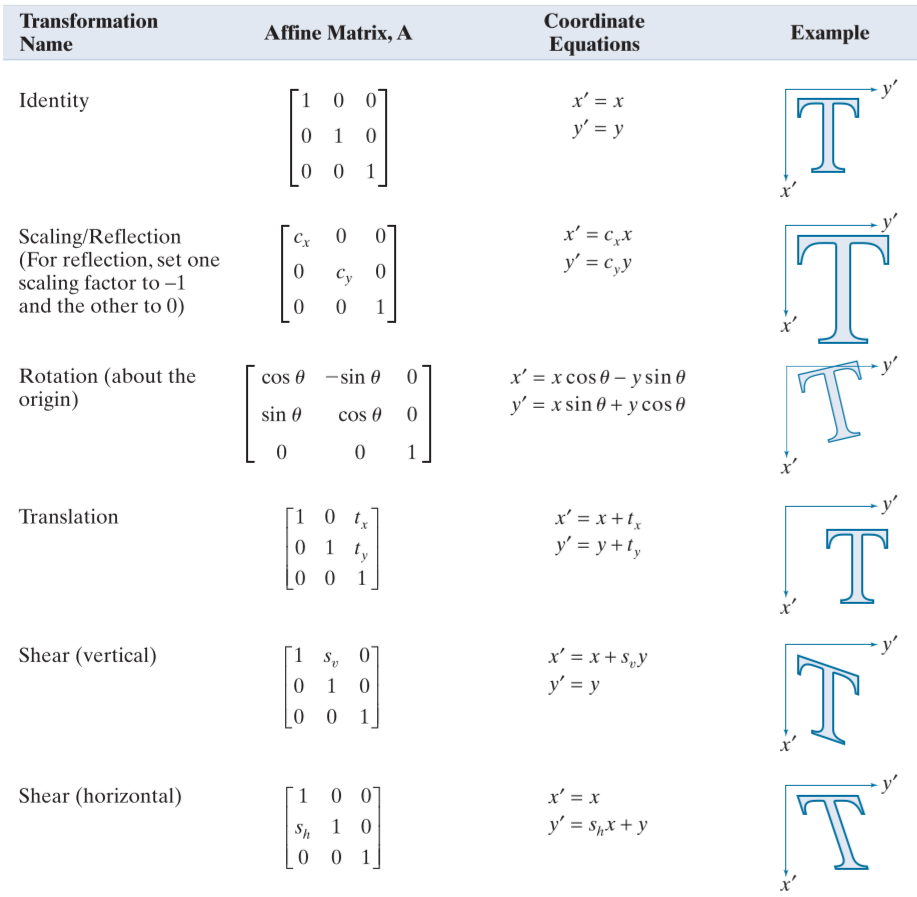
\includegraphics[width=\linewidth]{trans.png}
\end{columns}
\end{frame}

% Contents Frame
\begin{frame}{Contents}
\begin{itemize}
    \item \textbf{Introduction and Fundamentals}: What is image registration, real-world applications, and core components.
    \item \textbf{Registration Paradigms}: Feature-based vs. Intensity-based approaches.
    \item \textbf{Feature-based Registration}: Keypoint detectors (Harris, SIFT, ORB), descriptors, matching strategies, and robust optimization (RANSAC).
    \item \textbf{Intensity-based Registration}: Spatial transformations, interpolation methods, similarity metrics (SSD, CC, Mutual Information), and ITK optimization frameworks.
    \item \textbf{Practical Guidelines}: How to select and execute the right registration pipeline.
\end{itemize}
\end{frame}

% ==========================================
% SECTION 1: INTRODUCTION & FUNDAMENTALS
% ==========================================
\section{Introduction and Fundamentals}
\begin{frame}
\centering
\vspace{0.25\textheight}
{\Huge Section 1: Introduction and Fundamentals}
\end{frame}

\begin{frame}{What is Image Registration?}
\begin{columns}[T,onlytextwidth]
\column{0.55\textwidth}
\textbf{Definition}:
\begin{itemize}
    \item The process of establishing spatial correspondences between two or more images of the same scene taken at different times, from different viewpoints, and/or by different sensors.
    \item Mathematically: Find a coordinate transformation $T$ that maps points in a \textit{moving image} $I_M$ to points in a \textit{fixed reference image} $I_F$ such that:
    \[
    I_M(T(\mathbf{x})) \approx I_F(\mathbf{x})
    \]
    for all spatial locations $\mathbf{x}$.
\end{itemize}
\column{0.41\textwidth}
\centering
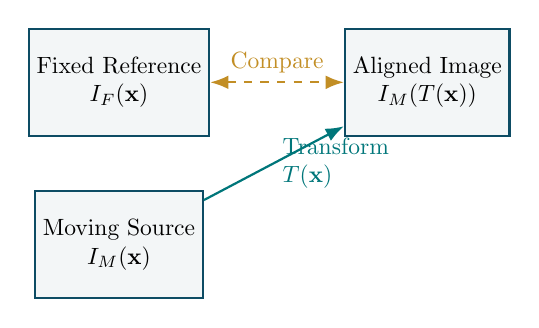
\begin{tikzpicture}[node distance=0.8cm, >=Latex, scale=0.85, every node/.style={transform shape}]
    \tikzstyle{img}=[draw=LectureBlue, thick, minimum width=2.4cm, minimum height=1.6cm, fill=LectureBlue!5, align=center]
    \node[img] (fixed) {Fixed Reference\\$I_F(\mathbf{x})$};
    \node[img, below=of fixed] (moving) {Moving Source\\$I_M(\mathbf{x})$};
    \node[img, right=2.0cm of fixed] (aligned) {Aligned Image\\$I_M(T(\mathbf{x}))$};
    
    \draw[->, thick, LectureTeal] (moving) -- node[right, align=left] {Transform\\$T(\mathbf{x})$} (aligned);
    \draw[dashed, <->, thick, LectureGold] (fixed) -- node[above] {Compare} (aligned);
\end{tikzpicture}
\end{columns}
\end{frame}

\begin{frame}{Applications: Temporal Monitoring (Monomodal)}
\begin{columns}[c,onlytextwidth]
\column{0.55\textwidth}
\textbf{Temporal Monitoring (Monomodal)}:
\begin{itemize}
    \item Aligning images of the same patient taken at different times using the same modality.
    \item \textbf{Use Case}: Tracking disease progression or treatment response (e.g., measuring tumor growth or shrinkage in brain MRI scans taken months apart).
    \item Ensures that differences observed are due to biological changes, not patient alignment or positioning errors.
\end{itemize}
\column{0.41\textwidth}
\centering
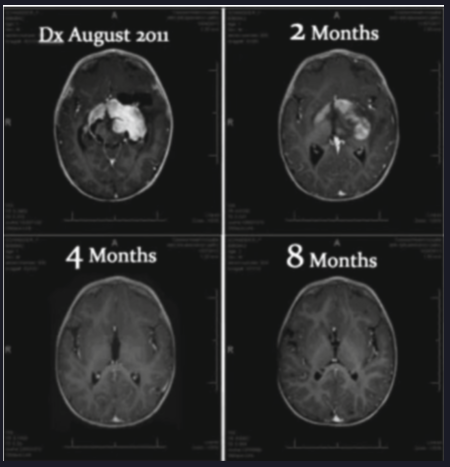
\includegraphics[width=\linewidth]{application_temporal_monitoring.png}
\end{columns}
\end{frame}

\begin{frame}{Applications: Multimodal Fusion}
\begin{columns}[c,onlytextwidth]
\column{0.55\textwidth}
\textbf{Multimodal Fusion}:
\begin{itemize}
    \item Aligning two or more images of different modalities (e.g., PET, CT, MRI) for the same patient.
    \item \textbf{Use Case}: Combining anatomical details (from CT/MRI) and functional/metabolic information (from PET) to assist in diagnosis and planning.
\end{itemize}
\column{0.41\textwidth}
\centering
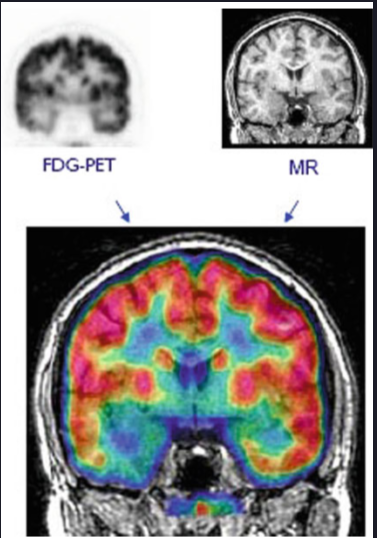
\includegraphics[width=\linewidth]{application_multimodal_fusion.png}
\end{columns}
\end{frame}

\begin{frame}{Applications: Landmark-based Registration}
\textbf{Landmark-based Registration}:
\begin{itemize}
    \item Used when images are highly distorted, undergo large deformations, or lack clear global intensity correlation.
    \item \textbf{Use Case}: Aligning images by manually or semi-automatically identifying matching physical landmarks (markers, anatomical landmarks).
\end{itemize}

\centering
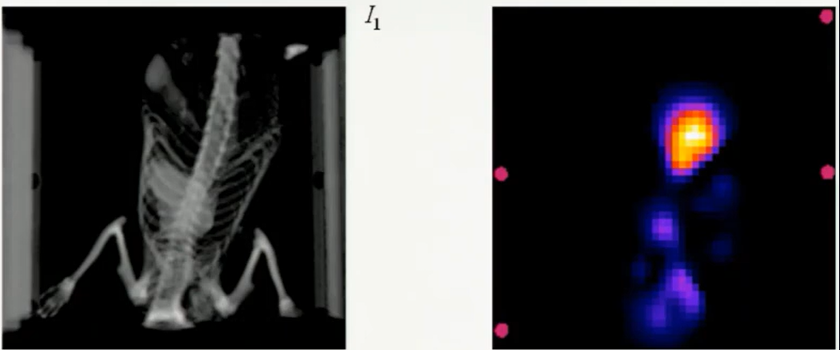
\includegraphics[width=0.7\linewidth]{application_landmark_registration.png}
\end{frame}

\begin{frame}{The Four Core Components}
Any registration framework is characterized by a combination of four distinct elements:
\begin{enumerate}
    \item \textbf{Transformation Model ($T$)}: Defines how coordinates are mapped from one image space to another (e.g., Rigid, Affine, Deformable).
    \item \textbf{Similarity Metric ($S$)}: Quantifies the quality of alignment. It acts as the objective function (or loss function) to be minimized or maximized.
    \item \textbf{Interpolator}: Reconstructs continuous intensities. Since transformed coordinates $T(\mathbf{x})$ generally fall off the discrete voxel grid, we must interpolate values.
    \item \textbf{Optimizer}: Search strategy that updates the parameters of the transformation model to find the best metric value.
\end{enumerate}
\end{frame}

% ==========================================
% SECTION 2: PARADIGMS
% ==========================================
\section{Registration Paradigms}
\begin{frame}
\centering
\vspace{0.25\textheight}
{\Huge Section 2: Registration Paradigms}
\end{frame}

\begin{frame}{Feature-based vs. Intensity-based Paradigms}
\small
\begin{tabularx}{\textwidth}{l >{\raggedright\arraybackslash}X >{\raggedright\arraybackslash}X}
\toprule
\textbf{Dimension} & \textbf{Feature-based Methods} & \textbf{Intensity-based Methods} \\
\midrule
\textbf{Data Utilized} & Sparse local features (corners, edges, keypoints). & Global intensity values across all voxels in ROI. \\
\textbf{Computational Cost} & Fast matching once features are extracted. & Computationally heavy (evaluates similarity metrics globally). \\
\textbf{Preprocessing} & High (requires detection, descriptor extraction, and outlier removal). & Low (mainly intensity normalization, resampling). \\
\textbf{Locality} & Local. Computes correspondences from distinct local neighborhoods. & Global. Uses statistical properties of the entire image. \\
\textbf{Robustness} & Robust to huge geometric shifts/rotations. & Susceptible to local minima; needs good initialization. \\
\bottomrule
\end{tabularx}
\end{frame}

\begin{frame}
    \centering
    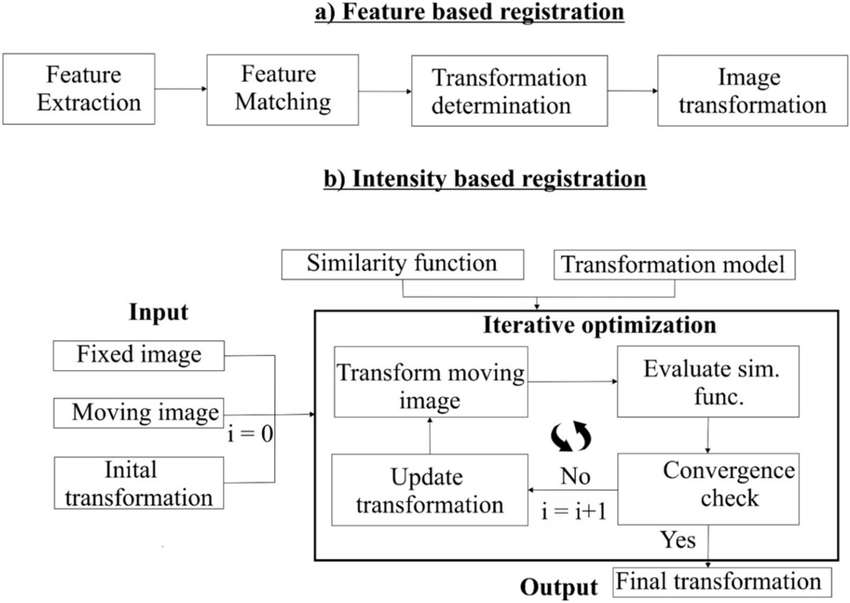
\includegraphics[width=0.8\textwidth]{features_vs_intensity.png}
\end{frame}

\begin{frame}{Feature-based Example: Manual Point Mapping}
    \textbf{Manual Point Mapping}:
    \begin{itemize}
        \item Ground control points (landmarks) are manually selected by a user in both images.
        \item \textbf{Example}: Registering aerial photos where features like road intersections, river bends, or building corners are matched.
        \item The transformation parameters are solved directly from these point pairs using a least-squares fit.
    \end{itemize}
    \vspace{0.5cm}
    \centering
    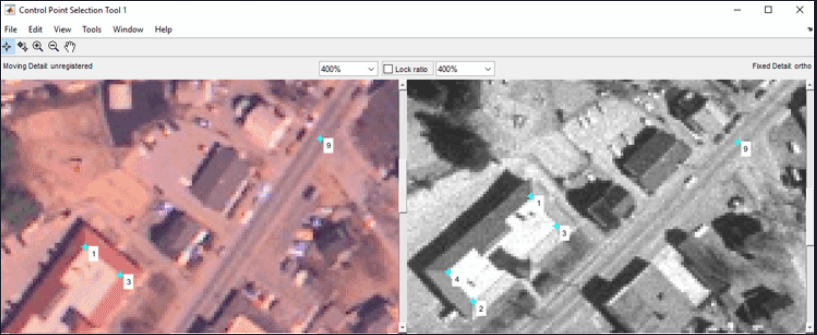
\includegraphics[width=0.8\linewidth]{features_based_ex1.png}
\end{frame}


\begin{frame}{Feature-based Example: Automatic Feature Matching}
    \textbf{Automatic Feature Matching}:
    \begin{itemize}
        \item Computer algorithms automatically detect distinct keypoints and extract descriptors.
        \item \textbf{Example}: Keypoints are detected, described, and matched between the fixed and moving images.
    \end{itemize}
    \vspace{0.5cm}
    \centering
    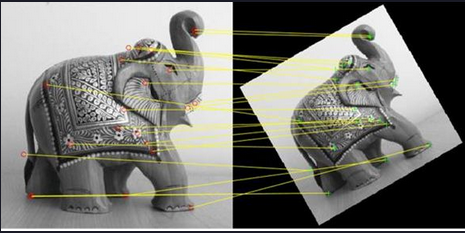
\includegraphics[width=0.8\linewidth]{features_based_ex2.png}
\end{frame}


\begin{frame}{Intensity-based Example}
    \textbf{Intensity-based Example}:
    \begin{itemize}
        \item Direct alignment of intensity patterns without feature detection or extraction.
        \item \textbf{Example}: Registering MRI and CT brain scans by maximizing statistical similarity.
        \item Uses all voxel intensities in the region of interest globally, adjusting the transform iteratively.
    \end{itemize}
    \vspace{0.5cm}
    \centering
    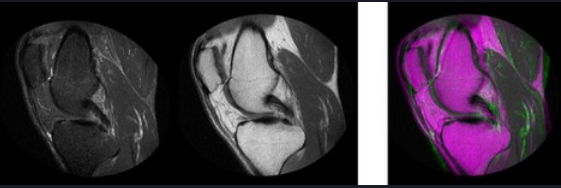
\includegraphics[width=0.8\linewidth]{intensity_based_ex1.png}
\end{frame}


% ==========================================
% SECTION 3: FEATURE-BASED METHODS
% ==========================================
\section{Feature-based Registration Algorithms}
\begin{frame}
\centering
\vspace{0.25\textheight}
{\Huge Section 3: Feature-based Registration Algorithms}
\end{frame}

\begin{frame}
    \centering
    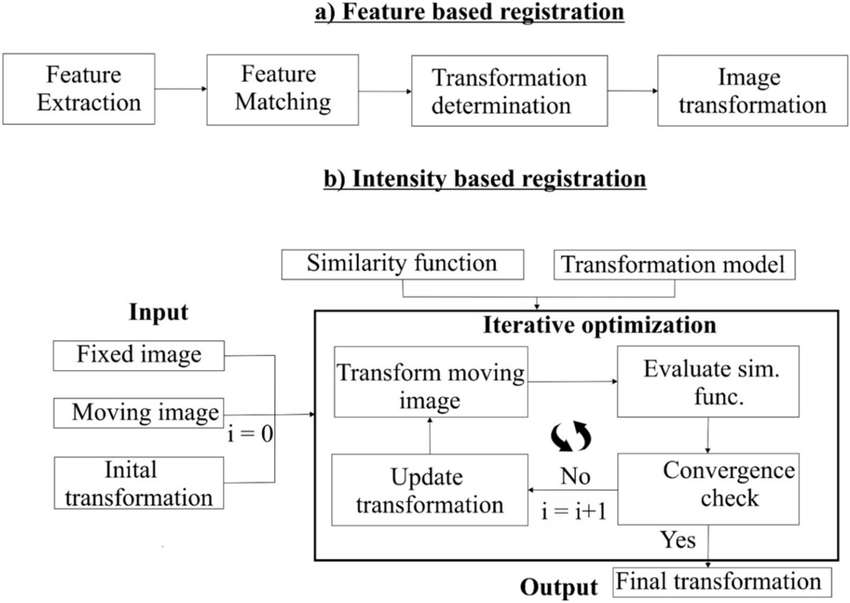
\includegraphics[width=0.8\textwidth]{features_vs_intensity.png}
\end{frame}

\begin{frame}{Feature Extraction: Detection and Description}
Feature-based image registration relies on a two-step feature extraction pipeline:
\vfill
\begin{block}{1. Keypoint Detection (``Where'')}
\begin{itemize}
    \item Locating distinct, highly repeatable interest points (e.g., corners, blobs, edges) in the image grid.
    \item \textbf{Examples}: Harris Corner Detector (detects corners only), FAST (detects corners), SIFT keypoints (detects scale-space blobs).
\end{itemize}
\end{block}
\vfill
\begin{block}{2. Feature Description (``What'')}
\begin{itemize}
    \item Constructing a robust numerical vector summarizing the local neighborhood around each keypoint.
    \item \textbf{Examples}: SIFT descriptor (128-D orientation histograms), BRIEF / ORB (binary tests matched via Hamming distance).
\end{itemize}
\end{block}
\end{frame}

\begin{frame}{Harris Corner Detector: Intuition}
\textbf{Basic Intuition}:
\begin{itemize}
    \item The detector shifts a small window (patch) in various directions to test for intensity variations.
    \item \textbf{Flat Region}: Moving the window in any direction results in no noticeable change in pixel intensities.
    \item \textbf{Edge}: Moving the window parallel to the edge yields no change; moving perpendicular yields a significant change.
    \item \textbf{Corner}: Moving the window in any direction yields a large change.
\end{itemize}

\centering
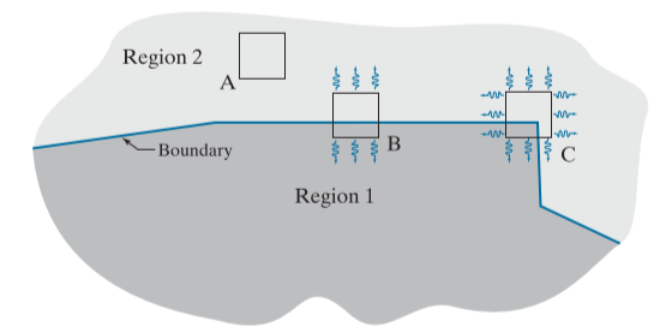
\includegraphics[width=0.8\linewidth]{harris_overview.png}
\end{frame}


\begin{frame}{Harris Corner Detector: Mathematical Formulation}
\begin{columns}[T,onlytextwidth]
\column{0.55\textwidth}
\small
\textbf{Concept}: Corners exhibit large intensity variations in all directions when shifted slightly.
\begin{itemize}
    \item Let $I(x,y)$ be the image intensity. The change in intensity for a shift $(u, v)$ is:
    \[
    E(u,v) = \sum_{x,y} w(x,y) \left[ I(x+u, y+v) - I(x,y) \right]^2
    \]
    where $w(x,y)$ is a windowing function (flat or Gaussian weight).
    \item Using a first-order Taylor expansion:
    \[
    I(x+u, y+v) \approx I(x,y) + I_x(x,y)u + I_y(x,y)v
    \]
    where $I_x = \frac{\partial I}{\partial x}$ and $I_y = \frac{\partial I}{\partial y}$.
\end{itemize}
\column{0.41\textwidth}
\centering
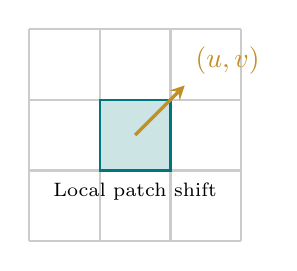
\begin{tikzpicture}[scale=0.9]
    \draw[thick, gray!40] (0,0) grid (3,3);
    \draw[fill=LectureTeal!20, draw=LectureTeal, thick] (1,1) rectangle (2,2);
    \draw[->, >=stealth, LectureGold, very thick] (1.5, 1.5) -- (2.2, 2.2) node[above right] {$(u,v)$};
    \node[font=\scriptsize] at (1.5, 0.7) {Local patch shift};
\end{tikzpicture}
\end{columns}
\end{frame}

\begin{frame}{Harris Corner Detector: Structure Tensor}
\small
Substituting the Taylor approximation back into the shift equation yields:
\[
E(u,v) \approx \sum_{x,y} w(x,y) \left[ I_x u + I_y v \right]^2 = \begin{bmatrix} u & v \end{bmatrix} M \begin{bmatrix} u \\ v \end{bmatrix}
\]
where $M$ is the symmetric $2\times 2$ \textbf{Structure Tensor} (or Second Moment Matrix):
\[
M = \sum_{x,y} w(x,y) \begin{bmatrix} I_x^2 & I_x I_y \\ I_x I_y & I_y^2 \end{bmatrix}
\]
The eigenvalues $\lambda_1$ and $\lambda_2$ of $M$ characterize the local structure of the patch:
\begin{itemize}
    \item \textbf{Flat region}: Both $\lambda_1, \lambda_2 \approx 0$ (no gradient).
    \item \textbf{Edge}: One eigenvalue is large, the other is near zero (gradient in one direction).
    \item \textbf{Corner}: Both $\lambda_1, \lambda_2$ are large (gradient in all directions).
\end{itemize}
\end{frame}

\begin{frame}{Harris Corner Detector: Response Function}
\small
Computing eigenvalues directly is computationally expensive. Harris proposed the corner response function $R$:
\[
R = \det(M) - k \text{Tr}(M)^2
\]
where $\det(M) = \lambda_1\lambda_2$, $\text{Tr}(M) = \lambda_1 + \lambda_2$, and $k$ is an empirical sensitivity factor ($0.04 - 0.06$).

\textbf{Classification rules}:
\begin{itemize}
    \item $R > \text{threshold}$: Corner ($\lambda_1, \lambda_2$ are both large).
    \item $R < -\text{threshold}$: Edge ($\lambda_1 \gg \lambda_2$ or vice versa).
    \item $|R|$ is small: Flat region.
\end{itemize}

\centering
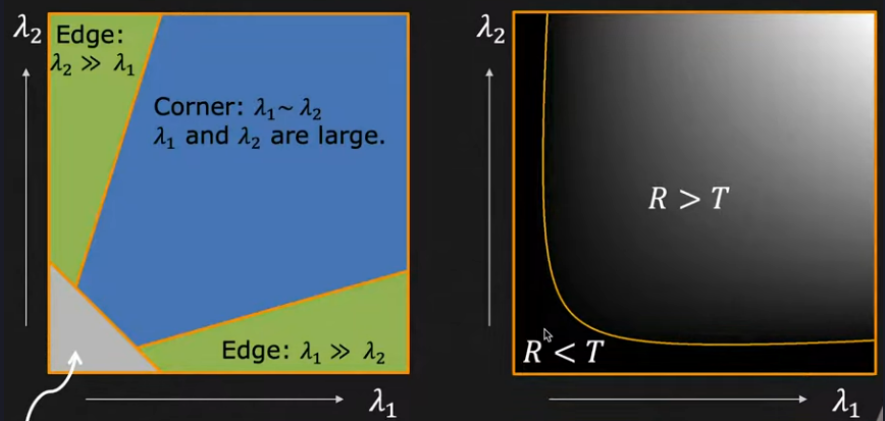
\includegraphics[height=0.5\textheight]{harris_decision.png}
\end{frame}

\begin{frame}{Scale-Invariant Feature Transform (SIFT)}

\textbf{Why Harris Fails under Scale}:
\begin{itemize}
    \item A corner in a fine-scale image may appear as a straight edge when zoomed in (magnified scale).
    \item SIFT solves this by searching for keypoints across both spatial scale and location.
\end{itemize}

\centering
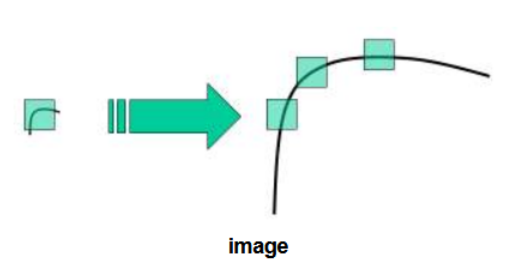
\includegraphics[width=0.7\linewidth]{sfit_idea.png}
\end{frame}

\begin{frame}{Scale-Invariant Feature Transform (SIFT)}


\centering
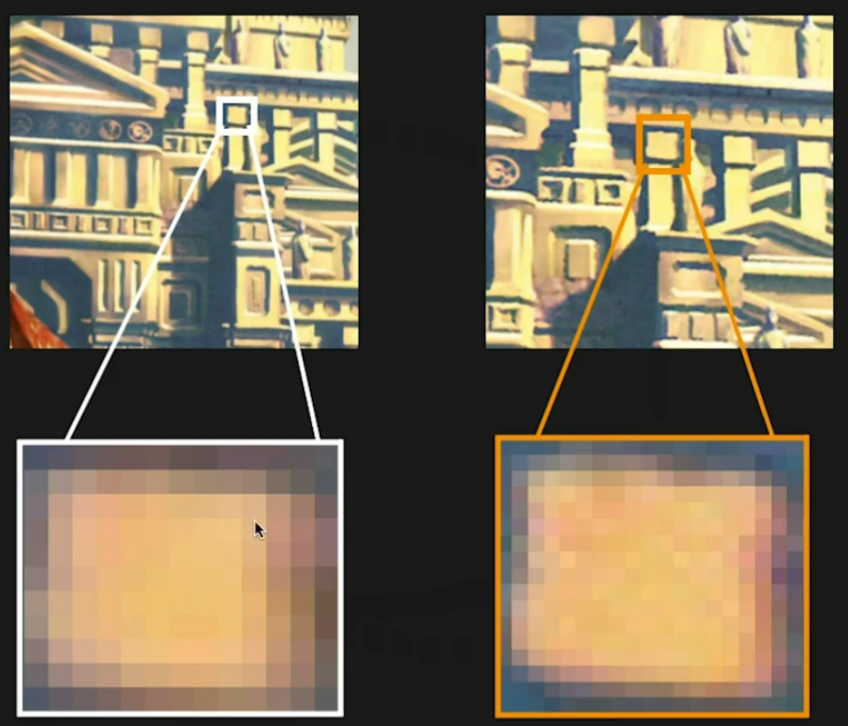
\includegraphics[width=0.6\linewidth]{sift_idea2.png}
\end{frame}

\begin{frame}{Scale Selection: Tuning the Feature Size}
How do we detect features of different sizes? We control the width of our derivative operator using the Gaussian parameter $\sigma$.

\begin{itemize}
    \item \textbf{Small $\sigma$ (Fine Scale)}: The Gaussian kernel is narrow. The derivative responds to sharp, localized changes—detecting fine-scale features (e.g., a tiny corner, a small pebble).
    \item \textbf{Large $\sigma$ (Coarse Scale)}: The Gaussian kernel is wide and blurs away fine details. The derivative operator expands, allowing it to detect large-scale features (e.g., a broad structure, an entire building).
\end{itemize}

\begin{block}{Derivative Theorem of Convolution}
Instead of blurring the image first and then computing the derivative, calculus allows us to take the derivative of the Gaussian kernel \textit{first}, and convolve that directly with the image:
\[
\frac{\partial^2}{\partial x^2} [L(x, y, \sigma)] = \frac{\partial^2}{\partial x^2} [G(x, y, \sigma) * I(x, y)] = \left[ \frac{\partial^2 G}{\partial x^2} \right] * I(x, y)
\]
\end{block}

\begin{center}
    \footnotesize{\textit{Varying $\sigma$ changes the physical size of the feature detector, matching the scale of the structures we wish to capture.}}
\end{center}
\end{frame}

\begin{frame}{Scale-Invariant Feature Transform (SIFT)}


\centering
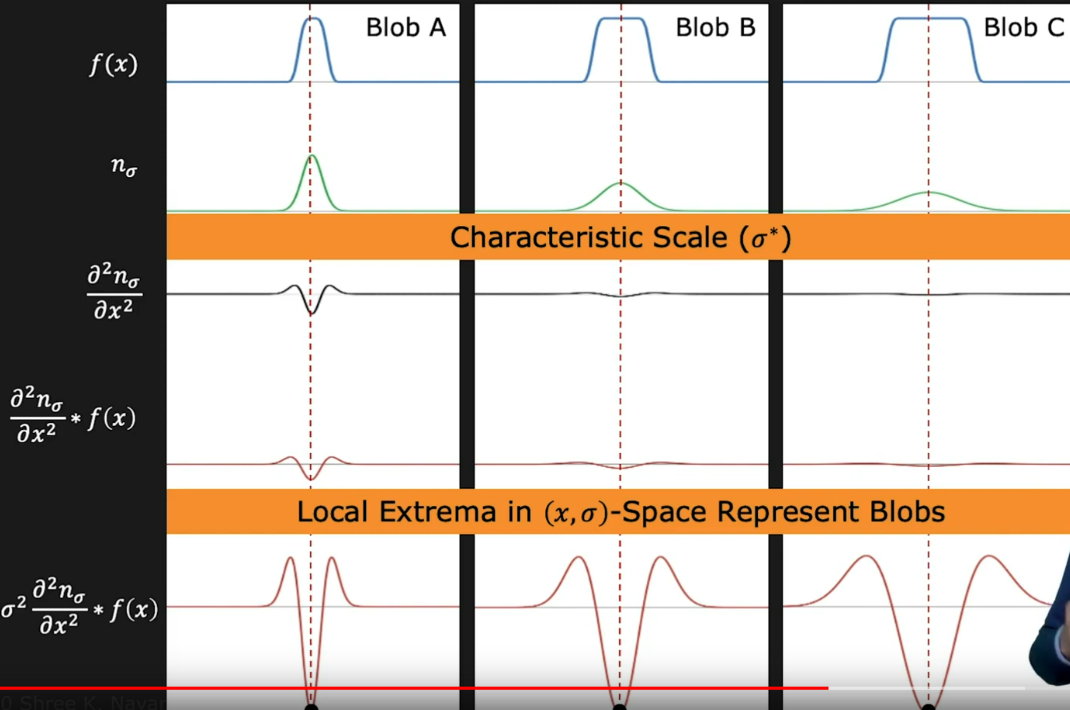
\includegraphics[height=0.85\textheight]{sift_gaussian.png}
\end{frame}

\begin{frame}{From Directional Derivatives to the Laplacian (LoG)}
The directional second derivative $\frac{\partial^2 G}{\partial x^2}$ only responds to intensity changes along the $x$-axis. We need a scale-tunable detector that is isotropic (responds equally in all directions).
\begin{itemize}
    \item For 2D image, we use Laplacian ($\nabla^2$):
    \[
    \nabla^2 L = \frac{\partial^2 L}{\partial x^2} + \frac{\partial^2 L}{\partial y^2}
    \]
    \item \textbf{Scale Normalization}: Because the amplitude of derivative responses naturally decays as $\sigma$ increases, we must multiply by $\sigma^2$ to compare feature strengths fairly across different scales:
\end{itemize}
\[
\text{Normalized LoG Response} = \sigma^2 \nabla^2 L = \sigma^2 \left( \frac{\partial^2 L}{\partial x^2} + \frac{\partial^2 L}{\partial y^2} \right)
\]
\end{frame}

\begin{frame}{Difference of Gaussians (DoG)}
\small
Convolving an image explicitly with a raw second-derivative LoG kernel at dozens of scales is computationally expensive. SIFT optimizes this using the **Difference of Gaussians (DoG)**.

\begin{block}{The Heat Diffusion Connection}
The derivative of a Gaussian scale-space with respect to scale ($\sigma$) matches its spatial second derivative (the Laplacian):
\[
\frac{\partial L}{\partial \sigma} = \sigma \nabla^2 L
\]
\end{block}

We approximate this continuous scale derivative $\frac{\partial L}{\partial \sigma}$ using a finite difference between two blurred images separated by a scale factor $k$:
\[
\frac{\partial L}{\partial \sigma} \approx \frac{L(x, y, k\sigma) - L(x, y, \sigma)}{k\sigma - \sigma} = \frac{D(x, y, \sigma)}{(k-1)\sigma}
\]

Substituting this approximation back into the heat equation yields the SIFT shortcut:
\[
D(x, y, \sigma) = L(x, y, k\sigma) - L(x, y, \sigma) \approx (k-1)\sigma^2 \nabla^2 L
\]
\end{frame}

\begin{frame}{Difference of Gaussians (DoG)}
\centering
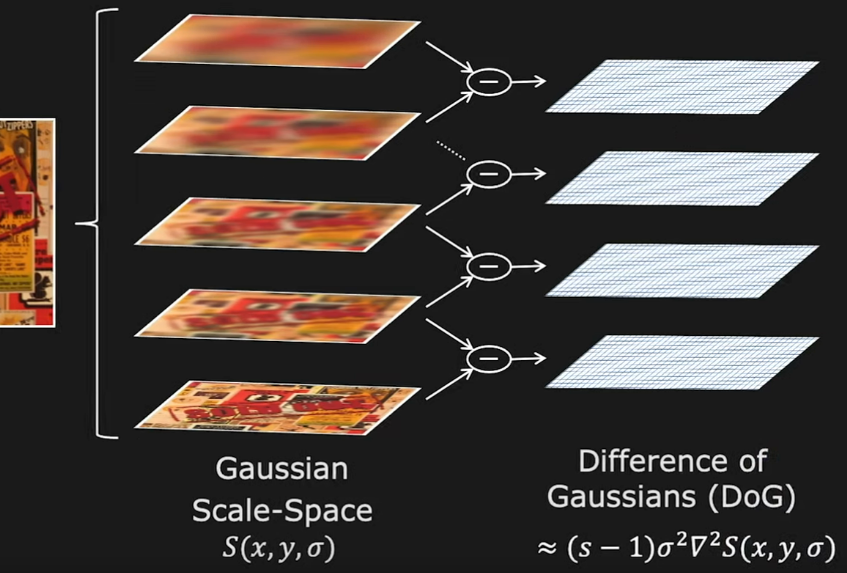
\includegraphics[width=0.7\linewidth]{sift_dog.png}
\end{frame}

\begin{frame}{Difference of Gaussians (DoG)}
\centering
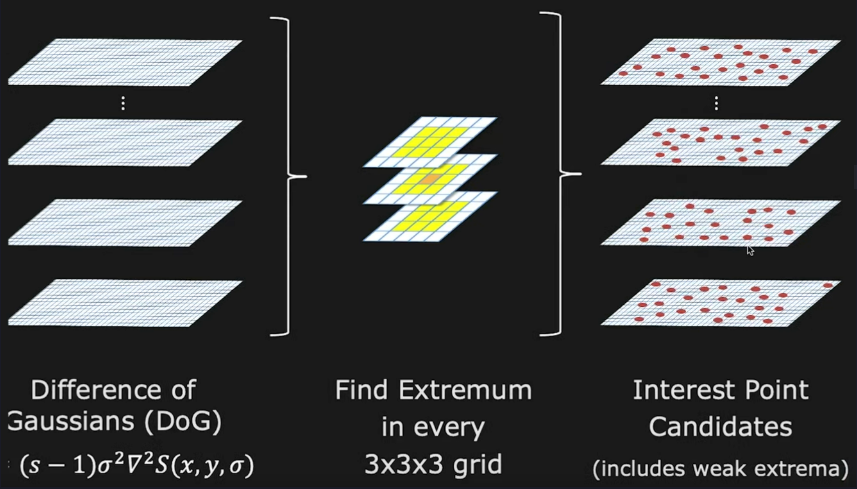
\includegraphics[width=0.8\linewidth]{sift_extrema.png}
\end{frame}

\begin{frame}{Difference of Gaussians (DoG)}
\centering
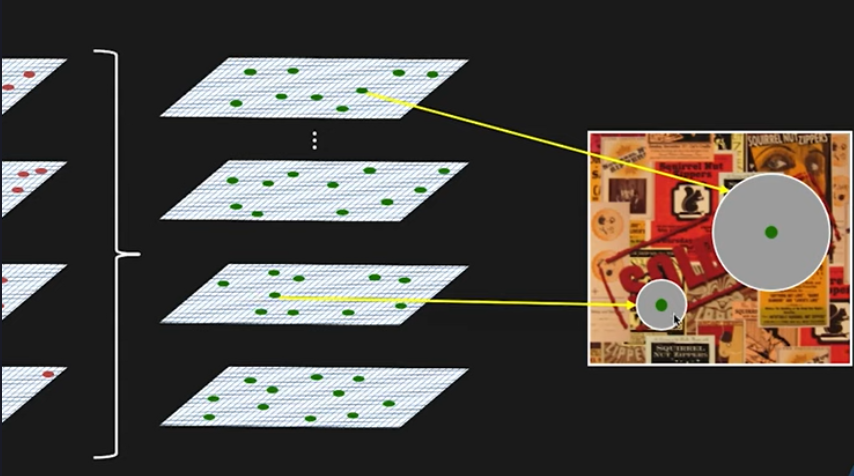
\includegraphics[width=0.8\linewidth]{sift_circle.png}
\end{frame}

\begin{frame}{Difference of Gaussians (DoG)}
\centering
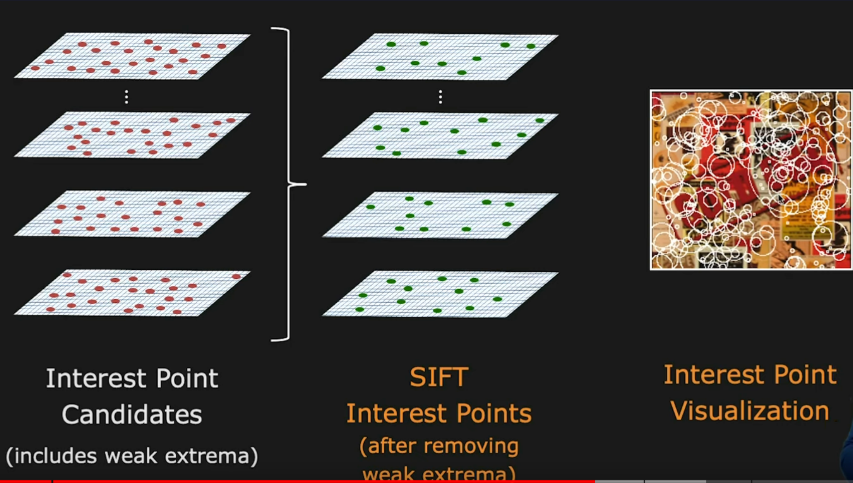
\includegraphics[width=0.8\linewidth]{sift_circle2.png}
\end{frame}

\begin{frame}{SIFT: Keypoint Descriptor}
Once a keypoint is localized (with a scale $\sigma$ and primary orientation $\theta$ for rotation invariance):
\begin{enumerate}
    \item \textbf{Orientation Alignment}: The coordinate system is rotated relative to $\theta$ to achieve rotation invariance.
    \item \textbf{Grid Sampling}: Gradient magnitudes and orientations are computed in a $16 \times 16$ spatial neighborhood around the keypoint.
    \item \textbf{Subgrid Histograms}: This neighborhood is divided into sixteen $4 \times 4$ subregions.
    \item \textbf{Vector Construction}: For each subgrid, an 8-bin orientation histogram is compiled. The resulting descriptor is a vector of size:
    \[
    16 \text{ subgrids} \times 8 \text{ bins/subgrid} = 128 \text{ values}
    \]
    This 128-D vector is normalized to unit length to provide illumination invariance.
\end{enumerate}
\end{frame}


\begin{frame}{SIFT Descriptor}
\centering
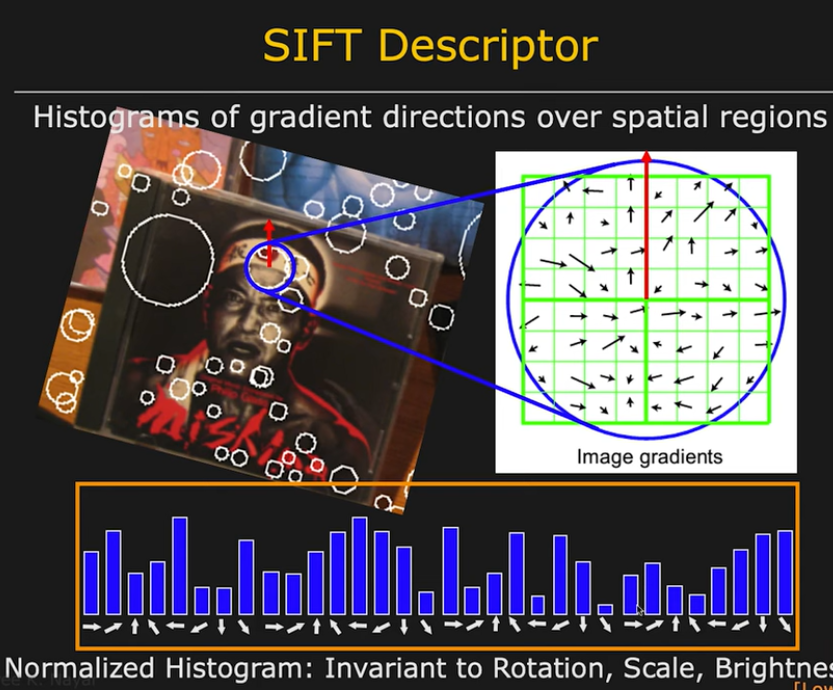
\includegraphics[width=0.6\linewidth]{sift_descriptor2.png}

\end{frame}

\begin{frame}{SIFT Descriptor}
\centering
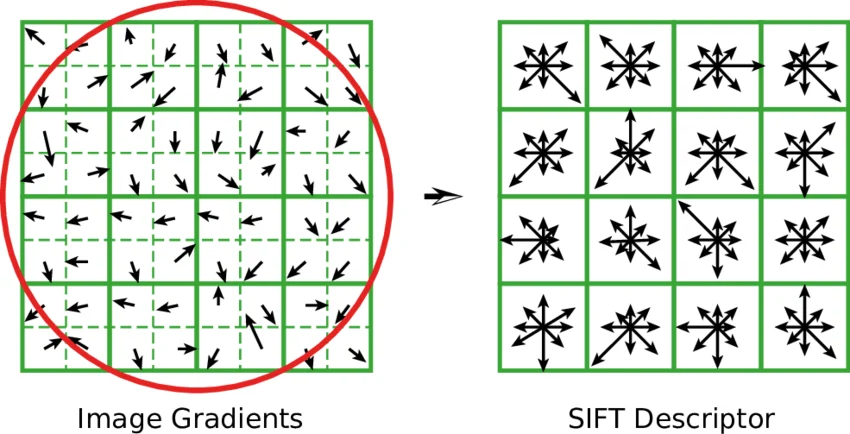
\includegraphics[width=0.8\linewidth]{sift_descriptor.png}
\footnotesize{\href{https://arxiv.org/abs/1604.08164}{https://arxiv.org/abs/1604.08164}}
\end{frame}

\begin{frame}{ORB: Oriented FAST and Rotated BRIEF}
SIFT is highly accurate but computationally expensive and patented for a long time. \textbf{ORB} is a fast, open-source alternative combining:
\begin{itemize}
    \item \textbf{oFAST (Oriented FAST)}:
    \begin{itemize}
        \item Keypoint detector based on comparing the intensity of a center pixel to a circle of 16 surrounding pixels.
        \item Computes the \textit{intensity centroid} of the local patch: $\mathbf{C} = \left(\frac{m_{10}}{m_{00}}, \frac{m_{01}}{m_{00}}\right)$, where $m_{pq} = \sum x^p y^q I(x,y)$ are moments.
        \item The vector from keypoint center to centroid defines the dominant orientation: $\theta = \operatorname{atan2}(m_{01}, m_{10})$.
    \end{itemize}
    \item \textbf{rBRIEF (Rotated BRIEF)}:
    \begin{itemize}
        \item Extracts binary descriptors using pairwise intensity tests.
        \item Pairs are rotated according to the keypoint's dominant orientation $\theta$.
        \item The descriptor is a bitstring of 256 bits, matched extremely fast using the Hamming distance.
    \end{itemize}
\end{itemize}
\end{frame}

\begin{frame}{Feature Matching Strategies}
Given descriptor sets $\{d_i^F\}$ and $\{d_j^M\}$ for the fixed and moving images:
\begin{itemize}
    \item \textbf{Brute-Force Matcher}: Computes distance (L2 for SIFT, Hamming for ORB) between every descriptor in set 1 and all descriptors in set 2. Returns the closest descriptor.
    \item \textbf{FLANN-based Matcher}: Uses fast nearest neighbor search trees (e.g., randomized KD-trees), highly effective for large datasets.
    \item \textbf{Lowe's Ratio Test}: Filtering ambiguous matches.
    \begin{itemize}
        \item A match is kept only if the ratio of the distance of the nearest neighbor ($d_1$) to that of the second-nearest neighbor ($d_2$) satisfies:
        \[
        \frac{d_1}{d_2} < \tau \quad (\text{typically } \tau \approx 0.75)
        \]
        This discards matches in repeated patterns where descriptors look similar.
    \end{itemize}
\end{itemize}
\end{frame}

\begin{frame}{Transformation Estimation and Robust Regression}
Given matched point coordinates $\{(\mathbf{x}_i, \hat{\mathbf{x}}_i)\}$, we fit a spatial transformation $f(\mathbf{x};\mathbf{p})$ with parameters $\mathbf{p}$.
\begin{itemize}
    \item \textbf{Ordinary Least Squares (OLS)}:
    \[
    E(\mathbf{p}) = \sum_i \left\| f(\mathbf{x}_i; \mathbf{p}) - \hat{\mathbf{x}}_i \right\| ^2
    \]
    OLS assumes errors are normally distributed. It is highly sensitive to mismatched features (outliers).
    \item \textbf{Robust Loss (M-estimators)}: Minimizes a robust penalty function $\rho$:
    \[
    E(\mathbf{p}) = \sum_i \rho\left( \left\| f(\mathbf{x}_i; \mathbf{p}) - \hat{\mathbf{x}}_i \right\| \right)
    \]
    Solved using Iteratively Reweighted Least Squares (IRLS), where weights are computed as $w_i = \rho'(r_i)/r_i$.
\end{itemize}
\end{frame}

\begin{frame}{RANSAC (Random Sample Consensus)}
If the initial match set contains more than 50\% outliers, gradient-based methods will converge to local minima. \textbf{RANSAC} is the standard algorithm for outlier rejection:
\vfill
\begin{block}{RANSAC Algorithm Steps}
\begin{enumerate}
    \item \textbf{Hypothesize}: Select a random minimal subset of matches (e.g., 4 matches for homography, 3 for affine) needed to estimate parameters $\mathbf{p}$.
    \item \textbf{Model Estimation}: Compute the candidate transformation $f(\mathbf{x};\mathbf{p})$ from the subset.
    \item \textbf{Consensus}: Transform all other points in the dataset. Count how many point matches fall within a tolerance distance $\epsilon$ (these are the \textbf{inliers}).
    \item \textbf{Iterate}: Repeat steps 1--3 for $N$ iterations.
    \item \textbf{Refinement}: Keep the model parameters $\mathbf{p}^*$ that produced the maximum number of inliers, and re-estimate the final transform using OLS on all identified inliers.
\end{enumerate}
\end{block}
\end{frame}

% ==========================================
% SECTION 4: INTENSITY-BASED METHODS
% ==========================================
\section{Intensity-based Registration}
\begin{frame}
\centering
\vspace{0.25\textheight}
{\Huge Section 4: Intensity-based Registration}
\end{frame}

\begin{frame}{Intensity-based Optimization Loop}
\centering
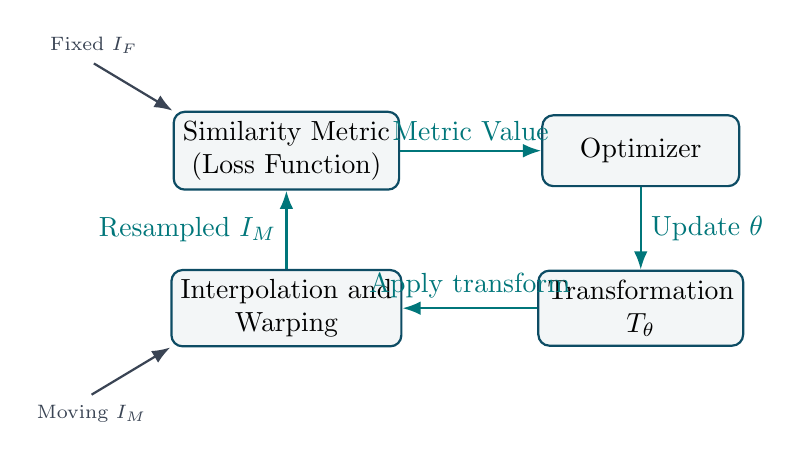
\begin{tikzpicture}[>=Latex,
    block/.style={draw=LectureBlue, rounded corners, thick, minimum width=2.5cm, minimum height=0.9cm, fill=LectureBlue!5, align=center}]
    
    \node[block] (metric) at (0,2) {Similarity Metric\\(Loss Function)};
    \node[block] (opt) at (4.5,2) {Optimizer};
    \node[block] (trans) at (4.5,0) {Transformation\\$T_\theta$};
    \node[block] (warp) at (0,0) {Interpolation and\\Warping};
    
    \draw[->, thick, LectureTeal] (metric) -- node[above] {Metric Value} (opt);
    \draw[->, thick, LectureTeal] (opt) -- node[right] {Update $\theta$} (trans);
    \draw[->, thick, LectureTeal] (trans) -- node[above] {Apply transform} (warp);
    \draw[->, thick, LectureTeal] (warp) -- node[left] {Resampled $I_M$} (metric);
    
    % Inputs
    \draw[<-, thick, Slate] (metric.north west) -- ++(-1.0, 0.6) node[above, font=\scriptsize] {Fixed $I_F$};
    \draw[<-, thick, Slate] (warp.south west) -- ++(-1.0, -0.6) node[below, font=\scriptsize] {Moving $I_M$};
\end{tikzpicture}
\end{frame}

\begin{frame}{Similarity Metrics: SSD and CC}
\begin{itemize}
    \item \textbf{Sum of Squared Differences (SSD)}:
    \[
    \text{SSD}(\theta) = \sum_{\mathbf{x} \in \Omega} \left[ I_F(\mathbf{x}) - I_M(T_\theta(\mathbf{x})) \right]^2
    \]
    \begin{itemize}
        \item \textbf{Assumption}: Identical image intensities up to Gaussian noise (monomodal matching).
        \item \textbf{Pros}: Simple, extremely fast derivative calculation.
        \item \textbf{Cons}: Sensitive to global contrast variations or modality changes.
    \end{itemize}
    \item \textbf{Cross-Correlation (CC)}:
    \[
    \text{CC}(\theta) = \frac{\sum_{\mathbf{x}} \left[ I_F(\mathbf{x}) - \bar{I}_F \right] \left[ I_M(T_\theta(\mathbf{x})) - \bar{I}_M \right]}{\sqrt{\sum_{\mathbf{x}} \left[ I_F(\mathbf{x}) - \bar{I}_F \right]^2 \sum_{\mathbf{x}} \left[ I_M(T_\theta(\mathbf{x})) - \bar{I}_M \right]^2}}
    \]
    \begin{itemize}
        \item \textbf{Assumption}: Linear relationship between intensities of the two images.
        \item \textbf{Pros}: Robust to linear changes in gain and bias.
    \end{itemize}
\end{itemize}
\end{frame}

\begin{frame}{Similarity Metrics: Mutual Information (MI)}
\small
For multimodal registration (e.g., aligning CT to MRI), intensity relationships are highly non-linear. \textbf{Mutual Information (MI)} is based on probability and information theory.
\begin{itemize}
    \item \textbf{Entropy} $H(X)$: Quantifies uncertainty of a random variable $X$ (image intensity distribution):
    \[
    H(X) = -\sum_{x} p(x) \log p(x)
    \]
    \item \textbf{Joint Entropy} $H(X, Y)$: Quantifies uncertainty in the combined system:
    \[
    H(X, Y) = -\sum_{x, y} p(x, y) \log p(x, y)
    \]
    \item \textbf{Mutual Information}: Quantifies the reduction in uncertainty of $X$ given knowledge of $Y$:
    \[
    I(X; Y) = H(X) + H(Y) - H(X, Y) = \sum_{x, y} p(x, y) \log \frac{p(x, y)}{p(x)p(y)}
    \]
\end{itemize}
Maximizing $I(X;Y)$ means aligning images so that their joint intensity histogram becomes as sharp (clustered) as possible, representing a strong statistical relationship.
\end{frame}

\begin{frame}{Spatial Transformation Models}
\small
\begin{tabularx}{\textwidth}{l c >{\raggedright\arraybackslash}l X}
\toprule
\textbf{Model} & \textbf{DoF (3D)} & \textbf{Preserves} & \textbf{Description} \\
\midrule
\textbf{Translation} & 3 & Orientation, distance & Shifts coordinates along axis directions. \\
\textbf{Rigid} & 6 & Distance, angles & Translation + Rotation. \\
\textbf{Similarity} & 7 & Angles, shape ratios & Rigid + Uniform scaling. \\
\textbf{Affine} & 12 & Parallelism, lines & Scale, translation, rotation, shearing. \\
\textbf{Deformable} & $\infty$ & Topologically soft & Non-linear local warping (B-Splines, displacements). \\
\bottomrule
\end{tabularx}
\vfill
\begin{block}{Homogeneous Coordinate Representation (Affine Example)}
\[
\begin{bmatrix} x' \\ y' \\ 1 \end{bmatrix} = \begin{bmatrix} a_{11} & a_{12} & t_x \\ a_{21} & a_{22} & t_y \\ 0 & 0 & 1 \end{bmatrix} \begin{bmatrix} x \\ y \\ 1 \end{bmatrix}
\]
Compositions of affine transformations correspond to direct matrix multiplication.
\end{block}
\end{frame}

\begin{frame}{Interpolation Methods}
\begin{columns}[T,onlytextwidth]
\column{0.55\textwidth}
\small
\textbf{Why Interpolate? (Backward Mapping)}:
\begin{itemize}
    \item To avoid holes, we warp by iterating over pixels in the \textit{destination grid} $\mathbf{x}_{\text{dest}}$, mapping back to source coordinates $\mathbf{x}_{\text{src}} = T^{-1}(\mathbf{x}_{\text{dest}})$.
    \item $\mathbf{x}_{\text{src}}$ usually contains fractional coordinates. We must interpolate intensity values from neighboring grid points.
\end{itemize}
\textbf{Common Kernels}:
\begin{itemize}
    \item \textbf{Nearest Neighbor}: Assigns value of closest grid pixel. Preserves discrete class labels. Discontinuous.
    \item \textbf{Bilinear/Trilinear}: Linear combination of $2^D$ neighbors. Smooth, but acts as a low-pass blur filter.
    \item \textbf{Bicubic/Spline}: Uses $4^D$ neighborhood. Continuous first derivatives. Better edge representation.
\end{itemize}
\column{0.41\textwidth}
\centering
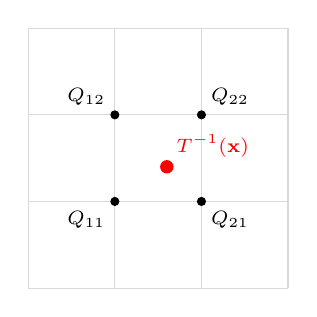
\begin{tikzpicture}[scale=1.1, font=\scriptsize]
    \draw[gray!30] (0,0) grid (3,3);
    \fill[black] (1,1) circle (1.5pt) node[below left] {$Q_{11}$};
    \fill[black] (2,1) circle (1.5pt) node[below right] {$Q_{21}$};
    \fill[black] (1,2) circle (1.5pt) node[above left] {$Q_{12}$};
    \fill[black] (2,2) circle (1.5pt) node[above right] {$Q_{22}$};
    
    \coordinate (P) at (1.6, 1.4);
    \fill[red] (P) circle (2.2pt) node[above right, red] {$T^{-1}(\mathbf{x})$};
\end{tikzpicture}
\end{columns}
\end{frame}

\begin{frame}{Optimizers and SimpleITK Framework}
\begin{columns}[T,onlytextwidth]
\column{0.55\textwidth}
\small
\textbf{Optimizers}:
\begin{itemize}
    \item Simple similarity metrics (SSD) have smooth derivatives, allowing standard Gradient Descent.
    \item Complex metrics (Mutual Information) have noisy, non-convex landscapes with multiple local minima.
    \item \textbf{Regular Step Gradient Descent}: Adjusts step size (shrinks it when gradient changes direction) to prevent oscillation.
\end{itemize}
\textbf{Multi-Resolution Framework}:
\begin{itemize}
    \item To avoid local minima, registration is often run in a coarse-to-fine pyramid (resolving major shifts first at low resolution).
\end{itemize}
\column{0.41\textwidth}
\centering
\includegraphics[width=\linewidth]{guideline.png}
\end{columns}
\end{frame}

% ==========================================
% SECTION 5: SUMMARY & GUIDELINES
% ==========================================
\section{Summary and Guidelines}
\begin{frame}
\centering
\vspace{0.25\textheight}
{\Huge Section 5: Summary and Guidelines}
\end{frame}

\begin{frame}{Practical Pipeline Selection Guide}
\centering
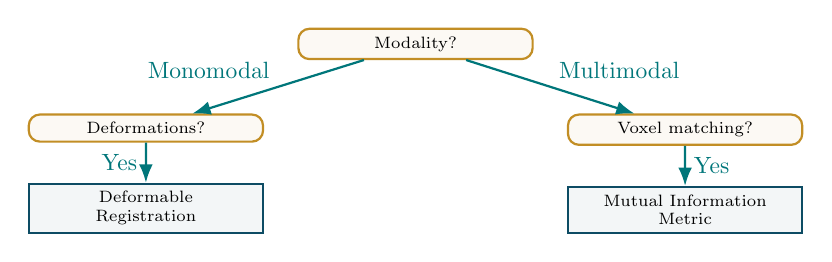
\begin{tikzpicture}[node distance=0.8cm, >=Latex, scale=0.85, every node/.style={transform shape}]
    \tikzstyle{q}=[draw=LectureGold, thick, rounded corners, fill=LectureGold!5, minimum width=3.5cm, align=center, font=\scriptsize]
    \tikzstyle{a}=[draw=LectureBlue, thick, fill=LectureBlue!5, minimum width=3.5cm, align=center, font=\scriptsize]
    
    \node[q] (q1) {Modality?};
    \node[q, below left=0.8cm and 0.5cm of q1] (q2a) {Deformations?};
    \node[q, below right=0.8cm and 0.5cm of q1] (q2b) {Voxel matching?};
    
    \node[a, below=0.6cm of q2a] (a1) {Deformable\\Registration};
    \node[a, below=0.6cm of q2b] (a2) {Mutual Information\\Metric};
    
    \draw[->, thick, LectureTeal] (q1) -- node[above left] {Monomodal} (q2a);
    \draw[->, thick, LectureTeal] (q1) -- node[above right] {Multimodal} (q2b);
    \draw[->, thick, LectureTeal] (q2a) -- node[left] {Yes} (a1);
    \draw[->, thick, LectureTeal] (q2b) -- node[right] {Yes} (a2);
\end{tikzpicture}
\vfill
\begin{itemize}
    \item \textbf{Use Feature-based} when: Initial alignments have large rotations/scale changes, or images contain easily detectable landmarks.
    \item \textbf{Use Intensity-based} when: Subtle, global structural alignments are needed, or when no distinct keypoints can be extracted reliably.
\end{itemize}
\end{frame}

\begin{frame}{Key Takeaways}
\begin{itemize}
    \item \textbf{Image Registration} is a mapping task $T: I_M \to I_F$.
    \item \textbf{Feature-based Methods} leverage sparse points (Harris corners, SIFT scale-space, ORB centroids) and use robust regression (RANSAC) to solve for $T$.
    \item \textbf{Intensity-based Methods} solve for $T$ by optimizing global similarity metrics (SSD, Cross-Correlation, Mutual Information).
    \item \textbf{Mutual Information} is the gold standard for multimodal registration as it measures statistical correlation rather than direct intensity values.
    \item \textbf{Interpolation} is a critical computational step needed for coordinate mapping during image warping.
\end{itemize}
\end{frame}

\end{document}
